\section{Framework}
We first introduce the procedure to extract positive event and its intervals from microblogs,
Based on this,
we present a statistical model to depict
the connection between positive events and adolescents' stress-buffering patterns through three groups of content and behavioral measures.
%Finally, a none-liner time series model was proposed to combine stress-buffering patterns into future stress prediction.
\subsection{Discovery of Positive Events from Microblogs}
\label{sec:frame1}
Let $u$ = $[type,\{doer, act,$ $description\}]$ be a positive event,
where the element \emph{doer} is the subject who performs the \emph{act},
and \emph{descriptions} are the key words related to $u$.
According to psychological scales ~\citep{Jun2008Influence,hassles},
adolescent positive events mainly focus on six dimensions,
as $\mathbb{U} =\{$ 'entertainment', 'school life', 'romantic', 'pear relationship', 'self-cognition', 'family life'$\}$. We constructed our lexicon for six-dimensional positive events from two sources.
The basic positive words are selected from the psychological lexicon C-LIWC (expectation, joy, love, surprise)~\citep{Tausczik2010The}.
Then we built six topic lexicons by expanding basic positive words from adolescent microblogs,
containing 452 phrases in 'entertainment',
273 phrases in 'school life',
138 phrases in 'romantic',
91 phrases in 'peer relationship',
299 phrases in 'self-recognition' and 184 phrases in 'family life', with totally 2,606 phrases,
as examples shown in table \ref{tab:topicWords}.
Additionally, we labeled \emph{doer} words (i.e., \emph{teacher}, \emph{mother}, \emph{I, we}) in positive lexicons.

\begin{table*}
\centering
\caption{\small{Topic words of six-dimensional positive events.}}
\label{tab:topicWords}
\small{
\begin{tabular}{lll}
\toprule
dimension & example words & total \\ \midrule
entertainment  & hike, travel, celebrate, dance, swimming, ticket, shopping, air ticket, theatre, party, Karaoke,& 452\\
                      & self-driving tour, game, idol, concert, movie, show, opera, baseball, running, fitness, exercise & \\
school life    & reward, come on, progress, scholarship,admission, winner, diligent, first place, superior & 273\\
				      & hardworking, full mark,  praise, goal, courage, progress, advance, honor, collective honor& \\
romantic       &  beloved, favor, guard, anniversary,  concern, tender, deep feeling, care, true love, promise, & 138\\
				      & cherish, kiss, embrace, dating, reluctant, honey, sweetheart, swear, love, everlasting, goddess &\\
pear relation  & listener, company, pour out, make friends with, friendship, intimate, partner, team-mate, brotherhood& 91\\
self-cognition & realize, achieve, applause, fight, exceed, faith, confidence, belief, positive, active, purposeful & 299\\
family life    & harmony, filial, reunite, expecting, responsible, longevity, affable, amiability, family, duty & 184\\
\bottomrule
\end{tabular}}
\end{table*}

\subsubsection{Linguistic Parser Model}
Positive events were identified through Chinese natural language processing platform \citep{Che2010}.
For each post, after word segmentation, we parsed each sentence to find its linguistic structure,
and then matched the main linguistic components with positive topic lexicons in each dimension.
The linguistic parser model was applied to identify the central verb of current sentence, namely the \emph{act}.
It constructed the relationship between the central verb and corresponding \emph{doer} and \emph{description} elements.
By searching these elements in positive topic lexicons,
the existence of positive events were identified.
Due to the sparsity of posts, the element \emph{act} might be empty.
\emph{Descriptions} were collected by searching all nouns, adjectives and adverbs.
Examples of positive events extracted from adolescents' microblogs are listed in table \ref{tab:uplifts}.
For the post 'Thanks all my dear friends hosting the party. Happiest birthday!!!',
it was processed as \emph{doer='friends', act = 'expecting', description = 'party'},
and \emph{type = 'entertainment'}.

\begin{table}
\begin{center}
\caption{\small{Extracted positive events from microblogs.}}
\small{
\begin{tabular}{|l|} \hline
I am really looking forward to the spring outing on Sunday now. \\
(doer:\emph{I}, act:\emph{looking forward}, description:\emph{spring outing})\\\hline
My holiday is finally coming [smile]. \\
(doer:\emph{My holiday}, act:\emph{coming}, description:\emph{[smile]})\\\hline
First place in my lovely math exam!!! In memory of it.\\
(description:\emph{first place, math, exam, memory})\\\hline
You are always here for me like sunshine. \\
(doer:\emph{You}, description:\emph{sunshine})\\\hline
Thanks all my dear friends hosting the party.
Happiest birthday!!!\\
(doer:\emph{friends}, act:\emph{thanks}, description:\emph{party, birthday})\\\hline
I know my mom is the one who support me forever, no matter \\
when and where. (doer:\emph{mom}, act:\emph{support})\\ \hline
Expecting Tomorrow' Adult Ceremony[Smile][Smile]~~\\
(act: \emph{expecting}, description:\emph{Adult Ceremony})\\\hline
\end{tabular}}
\label{tab:uplifts}
\end{center}
\end{table}

\subsubsection{Impact Intervals of Positive Events}
\label{subsec:interval}
We followed and extended ~\citep{Li2017Analyzing} to identify the impact interval of each positive event to further study its stress-buffering pattern.
Splitting interval is a common time series problem, and here we identified the target interval in three steps.

Step1:
Extracted positive events, stressor events and filtered out candidate intervals.
For each candidate interval,
we set its length to more than 3 days and a maximum gap of 1 day between two neighboured stressed days.
Since the stress series detected from microblogs were discrete points,
loess method was adopted to highlight characteristics of the stress curve.

Step2: Judged stressful intervals through hypothesis testing.
A Poisson based probability model was adopted to measure how confidently the current interval was a stressful interval.
Here the stressful posting rates under stress $\lambda_1$ and normal conditions $\lambda_0$ were modeled as two independent poisson process:
\begin{equation}
Pr[N=n|\lambda_i]=\frac{e^{-\lambda_i T}{(\lambda_i T)}^n}{n!}
\end{equation}
where $i\in\{0,1\}$, $n=0,1,\cdots,\infty$.
We expected that $\lambda_1 > \lambda_0$, and measured the probability as $P(\lambda_1>\lambda_0|N_1, T_1, N_0, T_0)$,
where $N_1, N_0$ are the number of stressful posts, and $T_1, T_0$ are time duration corresponding to $\lambda_1$ and $\lambda_0$.
Without loss of generality, we assume a Jeffreys non-informative prior on $\lambda_1$ and $\lambda_0$,
and inferred the posterior distribution $P(\lambda_1|N_1)$ and $P(\lambda_0|N_0)$ according to Bayes Rule.
Thus for current interval $I_1$ and historical normal interval $I_0$,
the quantified probability $\beta = P(\lambda_1>\lambda_0|I_1,I_0)$ $\in (0,1)$ indicated the confidence
whether $I_1$ was a stressful interval.

Step 3: Divided stressful intervals into SI set and U-SI set in temporal order.
For a detected stressful interval $I = <t_1,\cdots,t_n>$, we considered the temporal order between $I$ and any detected positive event $u$ happening at time point $t_u$ in three cases:
1) If the positive event $u$ happened during the stressful interval, i.e., $t_u \in [t_1,t_n]$, the positive interval $I$ was judged as $I \in U-SI$.
2) If the positive event happened nearby a stressful interval,
considering the probability that it conducted impact on current stressful interval.
Here the gap between $t_u$ and $I$ is limited to $\xi$, i.e.,
if $t_u \in [t_{1}-\xi, t_1)\cup(t_{n},t_{n}+\xi]$, then $I \in U-SI$.
If a stressful interval satisfies none of the above conditions, we classify it into the SI set.
3) Other stressful intervals were divided into U-SI set.

%M1: �������measure���㣬�ɴ˻���3��or4��
%M2: �Ƿ��б�Ҫ�ϲ�֮ǰ����ϸ������(��׸��)
\subsection{Relationship Between Positive Events and Adolescents' Microblogging Characteristics}
\label{sec:frame2}
%��ǰ���ӽ�
%�ӽ��
In our problem,
there were two sets of stressful intervals to compare:
the SI set and the U-SI set.
We formulated this comparison problem as finding the correlation between the two sets of multi-dimension points.
Each interval was modeled as a multi-dimensional vector according to the three groups of measures.
Specifically, we adopted the multivariate two-sample hypothesis testing method
\cite{Li2017Correlating,Johnson2012Applied} to model such correlation.
In this two-sample hypothesis test problem,
the basic idea is judging whether the multi-dimension points (i.e., stressful intervals)
in set SI and set U-SI were under different statistical distribution.
Assuming the data points in SI and U-SI were randomly sampled from distribution $F$ and $G$, respectively,
then the hypothesis was denoted as:
\begin{equation}
H_0: F = G \quad versus \quad H_1: F \neq G.
\end{equation}

\subsubsection{Statistical Model of Stress-buffering}

Under such hypothesis,
$H_0$ indicated points in SI and U-SI were under similar distribution,
while $H_1$ means points in SI and U-SI were under statistically different distributions,
namely positive events conducted obvious stress-buffering effect on current user.
Since each point in the two sets (SI and U-SI) was depicted in multi-dimensions,
here we took the KNN (K-Nearest Neighbor) based method \cite{Schilling1986Multivariate}
to judge the existence of significant difference between SI and U-SI.
For simplify, we used the symbol $A_1$ to represent set SI,
and $A_2$ represent set U-SI.
For each point $\ell_{x}$ in the two sets $A_1$ and $A_2$,
we expected its nearest neighbors (\emph{the most similar points}) belonging to the same set of $\ell_x$.

Three groups of behavioral measures (posting behavior,
stress change mode and linguistic expressions)
were indicated as \bm{${<D_p}$},\bm{${D_s}$},\bm{${D_l>}$}, respectively.
The Euclidean distance was adopted to calculate the distance of structured points in $A_1$ and $A_2$.
For each point $\ell x \in A=A_1\bigcup A_2$,
let $NN_r(\ell_x,A)$ be the function to find the $r-$th nearest neighbor of $\ell_x$.
Specifically, three sub-functions of $NN_r(.)$ are defined as $PNN_r(.)$, $SNN_r(.)$ and $LNN_r(.)$,
corresponding to user's linguistic expressions, stress change modes and posting behaviors in each stressful interval.
For point $\ell_x$ with linguistic expression matrix \bm{${D_l^x}$}, posting behavior matrix \bm{${D_p^x}$}
and stress change mode matrix \bm{${D_s^x}$},
the $r$-th nearest neighbor of $\ell_x$ in each measure was denoted as:
\begin{equation}
\begin{aligned}
& PNN_r(\ell_x,A)
= \{y | min\{||\textbf{D}_p^x-\textbf{D}_p^y ||_2\}, y\in(A/\ell_x)\} &\\
& SNN_r(\ell_x,A)
= \{z | min\{||\textbf{D}_s^x-\textbf{D}_s^z ||_2\}, z\in(A/\ell_x)\} \\
& LNN_r(\ell_x,A)
= \{w | min\{||\textbf{D}_l^x-\textbf{D}_l^w ||_2\}, w\in(A/\ell_x)\} &
 \end{aligned}
 \end{equation}
The $r$-th nearest neighbor considering all three groups of measures was denoted as:
\begin{align}
&NN_r(\ell_x,A) = \{v | min\{a \times ||\textbf{D}_p^x-\textbf{D}_p^v||_2+\\
&b \times ||\textbf{D}_s^x-\textbf{D}_s^v||_2+
c \times ||\textbf{D}_l^x-\textbf{D}_l^v||_2\}, v\in(A/\ell_x) \}
\end{align}
In this study, we set $a = b = c = 1/3$.
Next, let $I_r(\ell_x,A1,A2)$ be the function denoting whether the $r$-th nearest neighbor was in the same set with $\ell_x$:
\begin{equation}
I_r(\ell_x,A_1,A_2) =
\left\{ \begin{array}{ll}
1, \quad if \ell_x \in A_i  \&\& NN_r(\ell_x,A)\in A_i,\\
0, \quad otherwise
\end{array}
\right.
\end{equation}
Let $T_{r,n}$ denote the proportion that pairs containing two points from the same set among all pairs formed by $\ell_x \in A$
and its $k$ nearest neighbors:
\begin{equation}
T_{k,n}= \frac{1}{n\times k}\sum_{i=1}^{n}\sum_{j=1}^{k}I_j(x,A_1,A_2)
\end{equation}
The value of $T_{k,n}$ showed how differently the points in the two testing sets (SI and U-SI) performed.
If the value of $T_{r,n}$ was close to $1$,
it could be shown that the two underlying distributions $F$ and $G$ for $SI$ and U-SI were significantly different,
indicating current positive events conducted obvious stress-buffering impact on the teens' stress series.
Let $\lambda_1=|A_1|$ and $\lambda_2=|A_2|$, the statistic value $Z$ was denoted as:
\begin{align}
&Z=(nr)^{1/2}(T_{r,n}-\mu_{r})/\sigma_{r}\\
&\mu_r=(\lambda_1)^2+(\lambda_2)^2\\
&{\sigma_r}^2=\lambda_1\lambda_2+4{\lambda_1}^2{\lambda_2}^2
\end{align}
where $\mu_r$ was the expectation and ${\sigma_r}^2$ was the variance of $Z$.
Based on hypothesis test theory \cite{Johnson2012Applied},
when the size of the testing set ($\lambda_1$ and $\lambda_2$) were large enough,
$Z$ obeys a standard Gaussian distribution.
Thus we judged whether the positive events conducted significant stress buffering impact on the teen's stress series as follows:
if $f(SI,USI)=(nr)^{1/2}(T_{r,n}-\mu_{r})/{\mu_r}^2>\alpha$ ($\alpha = 1.96$ for $P=0.025$),
then the hypothesis $H_1$ was true.

%Linguistic expressions
\subsubsection{Measures}
\paragraph{Linguistic expressions}
Positive and stressful expressions were extracted from the post content.
The first linguistic measure was the frequency of \emph{positive emotional words},
which were identified based on four categories (surprise, joy, expectation, love) of LICW lexicons ~\citep{Tausczik2010The}.
The second measure was the frequency of \emph{positive event topic words} in six dimensions,
reflecting the existence of positive events (see table \ref{tab:topicWords} for examples).
Another important factor was wether existing \emph{self-mentioned words} (i.e., \emph{'I','we','my'}).
\citep{Li2014Major} showed that self-mentioned words exhibited high probability that the current event
was related to the author,
rather than the opinion about a public event or life events about others.
In addition to positive-related linguistic descriptions,
the frequency of \emph{stressor event topic words} in five dimensions
were adopted to represent the degree of attention for each type of stressor event.
The frequency of \emph{stressful emotional words}, based on four categories (anger, anxiety, hate, sad) of LICW lexicons, represented general stressful emotion during the interval.
For each student, we identified positive events in six dimensions applying the parser model in section \ref{sec:frame1}, and corresponding intervals based on algorithm in section \ref{subsec:interval}.
For intervals in two groups U-SI and SI,
Figure xx shows the distribution of above five measures in U-SI and SI.

\begin{figure}[h]
\centering
\includegraphics[width=\linewidth]{figs/gray/stopic.eps}
\caption{\small{Comparing topic words of five types of stressor events during stressful intervals in two situations:
1) intervals affected by neighboring positive events (U-SI), 2) no positive events occurred nearby (SI).}}
\label{fig:stopic}
\end{figure}

\begin{figure}[h]
\centering
\includegraphics[width=\linewidth]{figs/gray/utopic.eps}
\caption{\small{Comparing topic words of six types of positive events during stressful intervals in two situations:
1) intervals affected by neighboring positive events (U-SI), 2) no positive events occurred nearby (SI).}}
\label{fig:utopic}
\end{figure}


\begin{figure}[h]
\centering
\includegraphics[width=\linewidth]{figs/gray/topicAll.eps}
\caption{\small{Comparing stressful emotions and positive emotions during stressful intervals in two situations:
1) intervals affected by neighboring positive events (U-SI), 2) no positive events occurred nearby (SI).}}
\label{fig:topicAll}
\end{figure}


%all, positive, stressful
\paragraph{Posting behaviors}
Stress could lead to abnormal posting behaviors,
reflecting user's changes in social engagement activity ~\citep{Liang2015Teenagers}.
We considered three measures of posting behaviors in each time unit (day).
The first measure was \emph{posting frequency},
representing the total number of posts per day.
Research in \cite{Li2017Analyzing} indicated that overwhelmed adolescents tended to post more to express their stress for releasing and seeking comfort from friends.
The second measure was the \emph{positive posting frequency}, indicating the number of positive posts per day.
The third measure \emph{stressful posting frequency} per day highlighted the stressful posts among all posts.
Figure \ref{fig:post}shows the distribution of above three measures in U-SI and SI, respectively.

%The forth measure \emph{original frequency} was the number of original posts,
%which filtered out re-tweet and shared posts.
%Compared to forwarded posts, original posts indicated higher probability that users were talking about themselves.
%Thus in each interval, user's posting behavior was represented as a four-dimension vector.
\begin{figure}[h]
\centering
\includegraphics[width=\linewidth]{figs/gray/role.eps}
\caption{\small{Comparing role expressions during stressful intervals in two situations:
1) intervals affected by neighboring positive events (U-SI), 2) no positive events occurred nearby (SI).}}
\label{fig:role}
\end{figure}

\begin{figure}[h]
\centering
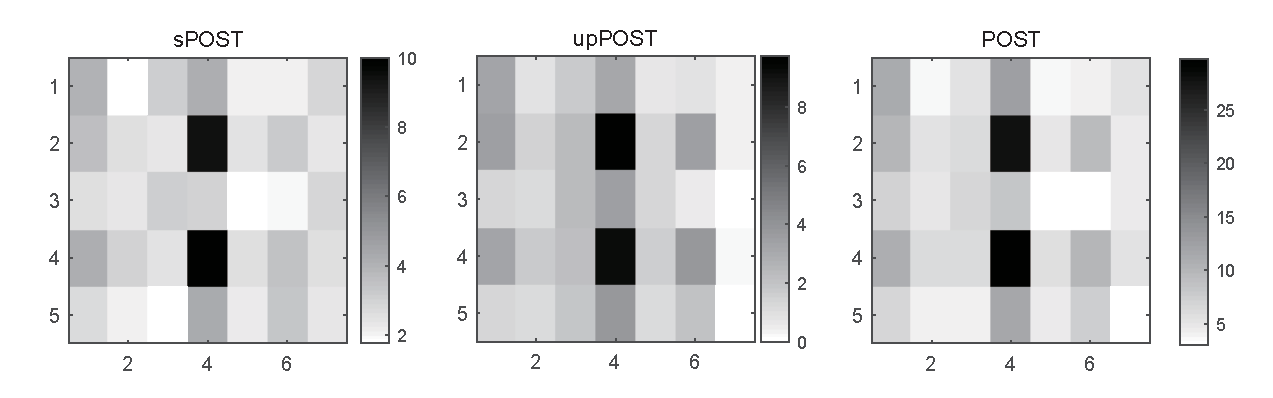
\includegraphics[width=\linewidth]{figs/gray/post.eps}
\caption{\small{Comparing posting behaviors during stressful intervals in two situations:
1) intervals affected by neighboring positive events (U-SI), 2) no positive events occurred nearby (SI).}}
\label{fig:post}
\end{figure}


\paragraph{Stress change modes}
Inspired by the pilot study,
the global stress change modes during a stressful interval were depicted through four measures:
\emph{sequential stress level, length of stressful interval, RMS value,} and \emph{maximal value}.
Basically, \emph{stress level} per day constructed a sequential measure during a stressful interval,
recording stress values and fluctuation on each time point.
As positive events might conduct impact on stressed adolescents,
and postpone the beginning or promote the end of a stressful interval,
we took \emph{length} as the second factor representing the interval stress change mode.
To quantify the intensity of stress fluctuations,
\emph{RMS} (root mean square) of stress values through the interval was adopted  as the third measure.
\emph{Peak} value was adopted as the forth measure to show the maximal stress value in current interval.
Next,
based on the above measures,
we quantified the difference between SI and U-SI sets, thus to track the stress-buffering pattern of positive events.
Figure \ref{fig:stress1,fig:stress2} exhibits eight stress change modes during SI and U-SI.
\begin{figure}[h]
\centering
\includegraphics[width=\linewidth]{figs/gray/stress1.eps}
\caption{\small{Comparing stress change modes during stressful intervals in two situations:
1) intervals affected by neighboring positive events (U-SI), 2) no positive events occurred nearby (SI).}}
\label{fig:stress1}
\end{figure}

\begin{figure}[h]
\centering
\includegraphics[width=\linewidth]{figs/gray/stress2.eps}
\caption{\small{Comparing stress change modes during stressful intervals in two situations:
1) intervals affected by neighboring positive events (U-SI), 2) no positive events occurred nearby (SI).}}
\label{fig:stress2}
\end{figure}



\subsubsection{Monotonous Model of Stress-buffering}
To verify the monotonous stress changes at both the early and late stress-buffering stages,
for each stressful interval in SI (n=2,582) and U-SI (n=1,914),
we compared its stress intensity with the front and rear adjacent intervals.
For a stressful interval $I = <t_i,t_{i+1},\cdots,t_j>$,
let $I^{front} = <t_m,\cdots,t_{i-1}>$ be the adjacent interval before $I$,
and $I^{rear} = <t_{j+1},\cdots,t_n>$ be the rear adjacent interval of $I$.
The length of $I^{front}$ and $I^{rear}$ are set to $|I|$.
For the set of stressful intervals $SI$ composed of $<I_1,I_2,\cdots,I_N>$,
the corresponding sets of adjacent front and rear intervals are denoted as $SI^{front}$ and $SI^{rear}$.
Similarly, for the set of stressful intervals $USI$ = $<UI_1,UI_2,\cdots, UI_M>$ impacted by positive events,
the corresponding sets of adjacent front and rear intervals are denoted as $USI^{front}$ and $USI^{rear}$.
We compare the intensity of stress changes in following four situations,
where $g(.)$ is the function comparing two sets: \\
1) $g(SI,SI^{front}$) returns if intensive change happens when stressful intervals begin.\\
2) $g(SI,SI^{rear}$) returns if stress changes intensively after the stressful intervals end.\\
3) $g(USI,USI^{front}$) returns if intensive change happens when stressful intervals affected by positive events appears.\\
4) $g(USI,USI^{rear}$) returns if stress changes intensively after stressful intervals affected by positive events end.

In our problem, taking the comparison between $SI$ and $SI^{rear}$ for example,
the basic computation element $I_k \in SI \cup SI^{rear}$ in both sets is a multi-dimension interval.
Here we adopt the t-test method as the intensity computation function $g(.)$.
%The t-test algorithm measures if intensive positive or negative monotonous correlation
%exists between two sample sets.
The function $g(.) = t_{score}$ $\in$ (-1,1) is represented as:

\begin{equation}
\small{g(SI,SI^{rear})}= \frac{\mu_{SI}-\mu_{SI^{rear}}}{\sqrt{\frac{(n_1-1)\sigma^2_{SI}+(n_2-1)\sigma^2_{SI^{rear}}}{n_1+n_2-2}(\frac{1}{n_1}-\frac{1}{n_2})}}
\end{equation}
where $\mu_{SI}$ and $\mu_{SI^{rear}}$ are the mean stress values of intervals in sets $SI$ and $SI^{rear}$,
and $\sigma_{SI}$ and $\sigma_{SI^{rear}}$ are the variance stress values of intervals in sets $SI$ and $SI^{rear}$, respectively.
If $g(SI,SI^{rear})$ $> \alpha$, stress intensity in $SI^{rear}$ show significant decrease compared with $SI$ (monotonic negative effect).
If $g(SI^{front},SI)$ $< -\alpha$, stress intensity in $SI$ show significant increase compared with $SI^{front}$ (monotonic positive effect).
Here we adopt $\alpha$ = 1.96, $P$ = 0.025.
We conduct comparison for above four situations,
to observe whether the occurrence of positive events relieve the monotonic negative effect of $g(SI,SI^{rear})$
and the monotonic positive effect of $g(SI^{front},SI)$.

